\documentclass{article}
\usepackage[utf8]{inputenc}
\usepackage[backend=biber,
style=numeric,
citestyle=numeric]{biblatex}
\usepackage{url}
\usepackage{csquotes}
\usepackage{pgfplots}
\usepackage{pgfplotstable}
\pgfplotsset{compat=1.7}
\usepackage{tikz}
\usepackage{hyperref}
\usepackage{graphicx}

\addbibresource{citations.bib}
\graphicspath{{images/}}

\title{Detecting Spurious Correlations in Image Annotations}
\author{Felix Möller}
\date{August 10th, 2021}

\begin{document}
%TODO: Paragraphs, scale of Figure 1
\maketitle
\tableofcontents
\newpage
\section{Abstract}
Neural networks and especially Convolutional Neural Networks (CNN) have revolutionized the field of computer vision in the recent years. While neural networks become more refined every year they also become more complex and difficult to interpret. However, interpretability is important because it allows researchers to investigate whether their models make their predictions by "learning from the right thing" or not. Surprisingly, recent research has shown that many models' predictions rely on so-called spurious correlations. In this report, I will present overview over the existing methods and compare them with regard to their usability. Next, I will show what should and what should not be done to mitigate the impact of spurious correlations on classification accuracy and finally I will propose a workflow to handle datasets that could contain spurious correlations. 
\section{Introduction}
\subsection{What is a spurious correlation (s.c.)?}
Before we have a look at the impact of spurious correlations on image datasets we first need to focus on what spurious correlations are. According to \cite{sc_def} a spurious correlation is a \enquote{connection between to variables that appears causal but is not}. This means that there \textit{appears} to be a logical explanation for the co-movement of both variables when the correlation is in fact completely random. The section \enquote{Why is detecting s.c.s in image datasets difficult?} mention why this is especially problematic in a machine learning context.
In this report, I will only have a look at spurious correlations that exist between a given feature of the dataset (e.g. the background of the image)and the target value (e.g. the age of a person) as these are the only spurious correlations that might cause the classifier to make wrong generalizations.

\subsection{Common types of s.c.s in image datasets}
Modern research has worked out two commonly occurring types of spurious correlations. The first one is  between \textbf{image angle} and \textbf{target} \cite{5995347}. In datasets that contain such a spurious correlation, the target is often shown from a similar angle (e.g. in an image dataset made up of cars all cars could be shown from the front) or in the same part of the image (e.g. most of the time the object of interest is in the centre of the image). Spurious correlations between image angle and target can be problematic because an image recognition model trained on a dataset which contains such a spurious correlation might struggle to classify the target object when it is shown from an angle that was not present in the training dataset. \\
The next commonly occurring spurious correlation between \textbf{context} and \textbf{target} \cite{Singh_2020_CVPR}. Spurious correlations between context and target occur in datasets where a non-target object co-occurs with the target object. One example would be cars which are commonly depicted with people. A classifier trained on a dataset with a spurious correlation between context and target might infer that the target value has to occur with its spuriously correlated non-target object. So in our car example, a classifier might only detect a car if a person is also present in the image.

\subsection{Why study spurious correlations?}
Datasets containing spurious correlations can significantly diminish the accuracy of a model compared to training on a dataset where no spurious correlations are present. Kim et al. have shown how much varying degrees of the same spurious correlations impact the classification accuracy of a model \cite{Kim_2019_CVPR}. They planted a spurious correlation between a digit and its color into the classic MNIST dataset \cite{mnist}, meaning they assigned a mean color to every digit in the training set and then drew from $N(mu_{digit},{\sigma^2}_{train})$ where $mu_{digit}$ is the mean color of the given digit and ${\sigma^2}_{train}$ is the variance of the normal distribution which was altered between iterations. The digits in the test dataset were assigned a random color (i.e. the mean color was not digit-specific), indicating that there is no spurious correlation in the test dataset. The degree of the spurious correlation between digit and color in the training set depends on ${\sigma^2}_{train}$ with a low value indicating a high degree of the spurious correlation and vice-versa. The evaluation results can be seen in  \hyperref[fig:mnistGraph]{Figure 1}. Although the spurious correlation would most likely be noticed in practice for very low $\sigma^2$, it is clear to see that even for the highest $\sigma^2$ the drop in classification accuracy is still significant (keep in mind that state-of-the-art classifiers can easily obtain above 95 \% test accuracy on the MNIST dataset \cite{mnist_web}).

\begin{figure}
    \centering
    \begin{tikzpicture}[scale=0.8]
    \begin{axis}[
        xlabel = $\sigma^2$,
        ylabel = Accuracy,
        width=10cm,
        height=7cm,
    ]
    \addplot[color=red, mark=.] coordinates {
        (0.02,0.4)
        (0.025,0.48)
        (0.03,0.6)
        (0.035,0.66)
        (0.04,0.73)
        (0.045,0.8)
        (0.05, 0.84)
    };
    \end{axis}
    \end{tikzpicture}
    \caption{Effect of a spurious correlation between color and digit on classification accuracy in the classic MNIST dataset. A lower variance indicates a more severe spurious correlation and vice-versa.}
    \label{fig:mnistGraph}
\end{figure}

\subsection{Why is detecting s.c.s in image datasets difficult?}
\label{sec:challenges}
Detecting spurious correlations in a given dataset is a challenge, regardless of whether the dataset contains
text data, plain numbers or images. The problem remains to evaluate if a given correlation is spurious or not.
Whilst determining the causality of a correlation is often easy for humans because they are able to make use of
their human intuition, computers would have to inspect an infinite amount of images to classify a correlation as
(not) spurious. However a machine-learning model only has a limited amount of data to train on and the training
set it is given could misrepresent the concept it is trained for (i.e. contain spurious correlations). 
In such a case, the model would most likely rely on the spurious correlation(s) which is present in the training set.
An additional challenge in the context of image datasets is feature-extraction. Determining the correlation
between a given feature of a dataset and the target attribute (e.g. the correlation between the presence of a special word
and target attribute) can be automated when the dataset contains text data. Extracting high-level features such as
the location of an object in an image or the image angle it is captured from would require training
an additional classifier to detect the concept. Such a classifier could however make its predictions by exploiting spurious
correlations which makes this way of feature-extraction unreliable.
The last option is to inspect the dataset manually. While this is the most reliable method to detect spurious correlations, the sheer size of modern image datasets (IMDB-WIKI: 523,000 images \cite{Rothe-ICCVW-2015}, MS COC0: 328,000 images \cite{lin2015microsoft}) makes manual detection of spurious correlations infeasible.

\section{Detecting spurious correlations}
Despite the significant negative impact of spurious correlations on classification accuracy,
detecting spurious correlations remains largely unexplored to this day.
Nevertheless researchers have proposed a handful of algorithms to detect spurious correlations
in image datasets. These can be grouped into two categories: The first one is \textbf{human-based detection}
which relies on inspecting a dataset manually to detect spurious correlations. Although I have mentioned that
manually inspecting image datasets is not feasible in \hyperref[sec:challenges]{Section 2.4},
there are algorithms which rely on humans to detect spurious correlations. One member of this category is
Crowdsourcing \cite{10.1145/3366423.3380063}, which makes use of volunteers to speed up the detection process and increase its reliability.
The second category is \textbf{Detection via model explanations}. Methods belonging to this category inspect a model trained on the given dataset to check if the model exploits spurious correlations to make its predictions. This can either be done by highlighting the parts of an image which contributed to the classification or by testing if the model responds to a user-defined concept. Gradient-weighted Class Activation Mapping (Grad-CAM) \cite{Selvaraju_2017_ICCV} makes use of the former, while Testing with concept activation vectors (TCAV) \cite{pmlr-v80-kim18d} relies on the latter.

\subsection{Crowdsourcing}
The main principle of Hu et al.'s Crowdsourcing approach \cite{10.1145/3366423.3380063} is to distribute the given dataset among all multiple volunteers to reduce the individual effort of each person. A brief summary of their approach can be seen in \hyperref[fig:crowdsourcing]{Figure 2}. \\
Their proposed algorithm consists of three steps: Step 1 is called \textbf{Question generation}. In this step each volunteer is provided with a random sample of the dataset. Next, each volunteer creates questions regarding anomalies he has found in his sample of the dataset where the answer to such a question is the given anomaly (the answer is also given by the volunteer). Between step 2 and step 1 all similar questions are merged via spaCy, an open-source natural language processing tool \cite{spaCy}. \\
In Step 2 which is called \textbf{Answer collection} the dataset is again randomly distributed among the volunteers of this step. Note that a volunteer only participates in one step of the process to increase its reliability. Among with a sample of the dataset a volunteer is confronted with question generated in step 1 which he answers with the anomaly he sees in his sample of the dataset. If the volunteer sees no anomaly in his sample, he can skip the question. Between steps 2 and 3 a weight $w_{i,2}$ is assigned to each potential spurious correlation $i$ which is the fraction of volunteers who provided the most common answer (similar answers to a question are merged). In addition, each question is transformed into a statement. \\
In Step 3 which is called \textbf{Bias Judgement} another group of volunteers is confronted with the statements generated at the end of step 2. Most importantly, the volunteers do not see the dataset. They then have to answer whether or not the given statements reflect the real world (yes/no answers only). At the end of step 3 another weight $w_{i,3}$ is assigned to each potential spurious correlation $i$ which is the fraction of workers stating that the statement belonging to a potential spurious correlation is not an accurate reflection of the real world. \\
After step 3, the total weight $W_{i}=w_{i,2} \cdot w_{i,3}$ is assigned to each potential spurious correlation the idea behind the computation of the total weight is that the severity of each potential spurious correlation is determined by how abnormal it is (determined in step 3)\textit{and} by how present it is in the dataset (determined in step 2). All spurious correlations with $W_i > t$ are the output of the algorithm where $t$ is a threshold which can be chosen by the conductors of the algorithm. \\
\begin{figure}
    \centering
    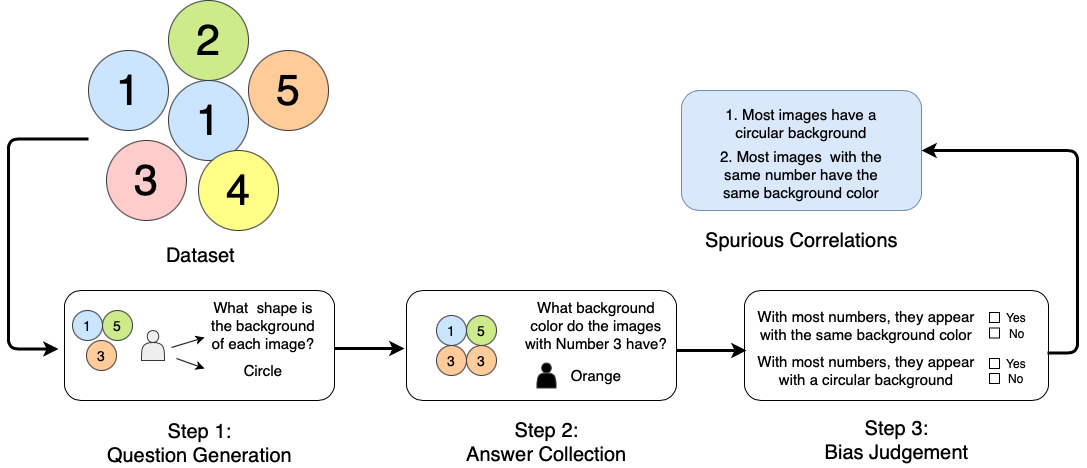
\includegraphics[scale=0.315]{crowdsourcing.png}
    \caption{Crowsourcing approach to detect spurious correlations in image datasets, proposed by Hu et al. \cite{10.1145/3366423.3380063}}
    \label{fig:crowdsourcing}
\end{figure}
In summary, Crowdsourcing can be seen as an effective algorithm because it largely relies on human intuition to detect spurious correlations. An additional benefit of this approach is that it is conducted by working directly on the dataset which makes it superior to model explanations. \\
In both studies conducted by Hu et al. more than 10 volunteers per 100 images took part in the study. Even if one were to inspect only a small fraction of the dataset, one would need in excess of 100 volunteers! The fact that Crowdsourcing relies on such a large amount of volunteers is ambivalent. On the one hand, relying on multiple volunteers decreases the bias towards the perceptions of a small group and leads to finding more spurious correlations. However to most people needing to inspect a dataset such a large group of volunteers is unattainable and relying on humans to detect spurious correlations is time-consuming. Another problem with Crowdsourcing is that the output often contains incorrect detections. In the second study conducted by Hu et al. in which the volunteers inspected a car dataset two of the top 10 outputs were \enquote{No cars have rust} and \enquote{Each car is fueled by gasoline}. \\
In conclusion, Crowdsourcing is an effective approach to detect spurious correlations in image annotations but the high amount of time and effort it requires make it only applicable to frequently used datasets.
\subsection{Grad-CAM}

\subsection{TCAV}
\subsection{Comparing existing methods to detect spurious correlations}

\section{Mitigating the impact of spurious correlations}
\subsection{Why increasing model size exacerbates spurious correlations}
\subsection{How to mitigate the impact of spurious correlations between context and target}

\section{How to deal with datasets that might contain spurious correlations}

\section{Conclusion}

\printbibliography

\end{document}
